\documentclass{article}
\usepackage{graphicx}
\usepackage{caption}
\usepackage{subcaption}
\usepackage{url}

\usepackage{amsmath}

\newcommand{\code}[1]{\texttt{#1}}
\renewcommand\refname{5  \hspace{4 mm}References}

\begin{document}

\title{CS 867: Displaying Multiple Time Series}
\date{December 16, 2013}
\author{Carmen St.\ Jean}

\maketitle

\section{Introduction}

Time-oriented data might be one of the most common forms of data, used in numerous fields such as medicine, economics, ecology, engineering, and meteorology.  Typically, time series are visualized using line charts, which appear frequently in newspapers, textbooks, and academic papers.  However, it can be difficult to display many concurrent time series at once in an understandable manner using a line chart.  Therefore, we have introduced a new visualization technique called a stacked graph, which we propose may be suitable for showing many time series---i.e., fifteen---at once.  To test the merits of our creation, we have evaluated the stacked graph against two existing methods---small multiples and horizon graphs.

\subsection{Background}

Since it was first introduced by William Playfair in 1786 \cite{playfair1786}, the line chart has been a popular choice for displaying temporal data.  However, it has its limitations when it comes to multiple time series.  To be plotted on a single chart, each time series must be distinctly colored and/or patterned; as the number of time series increases, it becomes more difficult to make each series visually distinct.  Even if each time series are designed uniquely, it may be difficult to distinguish two time series which have similar vales and overlap frequently.

\begin{figure}
        \centering
        \begin{subfigure}[b]{0.4\textwidth}
                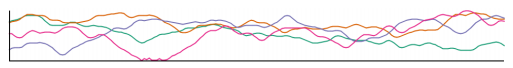
\includegraphics[width=\textwidth]{figures/ts_simplelinegraph.eps}
                \caption{A simple line graph.}
                \label{fig:ts_simple}
        \end{subfigure}
        \begin{subfigure}[b]{0.4\textwidth}
                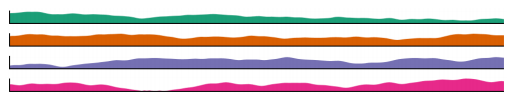
\includegraphics[width=\textwidth]{figures/ts_smallmultiples.eps}
                \caption{Small multiples.}
                \label{fig:ts_smmult}
        \end{subfigure}
        \\
        \begin{subfigure}[b]{0.4\textwidth}
                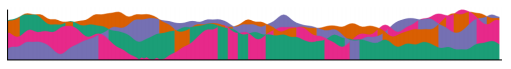
\includegraphics[width=\textwidth]{figures/ts_braidedgraph.eps}
                \caption{A braided graph.}
                \label{fig:ts_braid}
        \end{subfigure}
        \begin{subfigure}[b]{0.4\textwidth}
                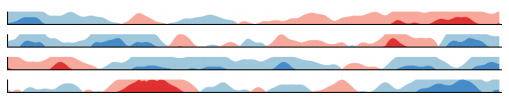
\includegraphics[width=\textwidth]{figures/ts_horizongraphs.eps}
                \caption{Horizon graphs.}
                \label{fig:ts_horizon}
        \end{subfigure}
        \caption{Four possible methods for visualizing multiple time series \cite{javed2010}.}
        \label{fig:ts_compare}
\end{figure}

Recognizing the limitations of the line chart for many time series leads to a question: what is a suitable alternative?  Javed et al.\ set out to answer this question with their evaluation that compared the line chart, as in Figure~\ref{fig:ts_simple}, with three alternative techniques  \cite{javed2010}.  The first alternative, called ``small multiples'' simply places each time series on its own line chart, shown in Figure~\ref{fig:ts_smmult}.  The screen space must be split with this approach, which leads to less resolution in the vertical direction.  Therefore, Javed et al.\ introduced a shared space approach called the ``braided graph'' seen in Figure~\ref{fig:ts_braid}, which attempts to be easier to read than a line chart by coloring the areas underneath the curves.  Additionally, Saito et al.'s horizon graph, as in Figure~\ref{fig:ts_horizon}, was included in the evaluation \cite{saito2005}.

\begin{figure}
        \centering
        \begin{subfigure}[b]{0.5\textwidth}
                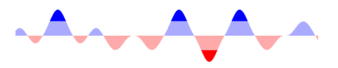
\includegraphics[width=\textwidth]{figures/construction1.eps}
                \caption{The line chart is divided into evenly-spaced bands, which are colored shades of blue in the upper-half and shades of red in the lower-half.}
                \label{fig:construction1}
        \end{subfigure}
        \\ 
        \begin{subfigure}[b]{0.5\textwidth}
                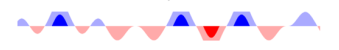
\includegraphics[width=\textwidth]{figures/construction2.eps}
                \caption{The bands of similar colors are layered together.}
                \label{fig:construction2}
        \end{subfigure}
        \\
        \begin{subfigure}[b]{0.5\textwidth}
                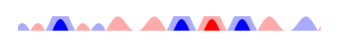
\includegraphics[width=\textwidth]{figures/construction3.eps}
                \caption{The red bands are mirrored.}
                \label{fig:construction3}
        \end{subfigure}
        \caption{Steps for constructing a horizon graph \cite{heer2009}.}
        \label{fig:hg_construction}
\end{figure}

Saito et al.\ designed horizon graphs to increase the amount of data that can be displayed without increasing graph size \cite{saito2005}.  To construct a horizon graph, some ``mid-line'' must be defined; it could represent zero or it could be the average of the global minimum and global maximum values in the dataset.  The areas between the mid-line and the data values are filled in, as in Figure~\ref{fig:construction1}, with blue for areas above the mid-line and red for areas below the mid-line.  The data is then further divided into evenly spaced bands, with the color of the band darkening as distance from the mid-line increases.  Next, these bands are offset to align with the mid-line, as in Figure~\ref{fig:construction2}.  Finally, the red bands are mirrored.  The result is the vertical resolution can be increased by a factor of four, as in Figure~\ref{fig:hg_construction}, or even more if more bands are used.

Javed et al.\ evaluated these four techniques illustrated in Figure~\ref{fig:ts_compare} by having participants complete three tasks on randomly-generated data:
\begin{enumerate}
	\item \textbf{Maximum:} for a given time point, identify the time series with the highest value
	\item \textbf{Slope:} for the entire time period, find the time series with the highest increase
	\item \textbf{Discrimination:} at a time point specific to each series, determine which series has the highest values
\end{enumerate}
In addition to chart type, their study varied the number of time series (2, 4, and 8) and the total chart height (48, 96, and 192 pixels).  They found that the simple line chart and the braided graph were best suited for the maximum task, while the small multiples and horizon graphs were better for the slope and discrimination tasks.  In general, they concluded that simple line charts and small multiples were generally more robust than horizon graphs and their newly introduced braided graphs. Additionally, they found that decreases in chart size did not affect completion time, but did decrease accuracy.  Lastly, as the number of concurrent time series increased, accuracy decreased and completion time increased. 

\section{Method}

Javed et al.'s approach considered only eight concurrent time series at most, when it is not unusual for many more to appear together in practice.  Therefore, we determined to conduct a similar study but with fifteen concurrent time series.  This number of time series makes simple line charts impractical, so they were not included in our evaluation.  Additionally, we decided to exclude braided graphs because they did not prove to be particularly effective in Javed et al.'s evaluation.  Instead, we have introduced stacked graphs, illustrated in Figure~\ref{fig:stackedGraph}, to compare with small multiples and line graphs, using data generated from a random walk.  We hypothesize that the stacked graph will prove to be a strong alternative for displaying many time series.

\subsection{Design}

\begin{figure}[h]
	\centering
	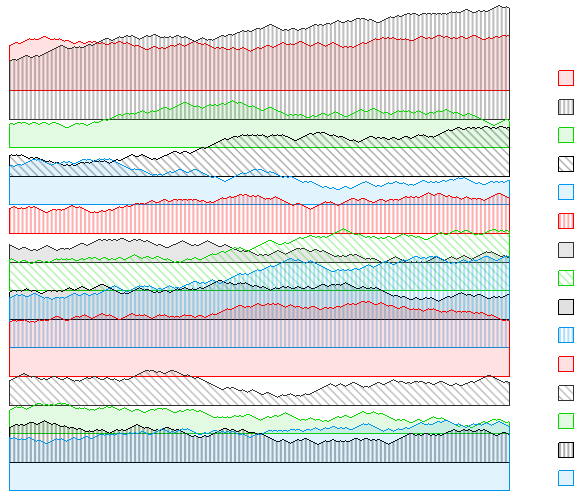
\includegraphics[width=6.5cm]{figures/stacked-new.eps}
	\caption{Fifteen time series represented with stacked graphs.}
	\label{fig:stackedGraph}
\end{figure}

Stacked graphs are called so because each time series is vertically-offset from the preceding time series, resulting in a stacked appearance.  An $x$-axis and a $y$-axis are drawn for each chart, though the latter is aligned for all charts.  We chose to use an offset of one-fourth of the individual chart height, which means that, at any point, a chart may overlap three other charts.  Therefore, we chose to fill the areas under each time series with semi-transparent, alternating colors and textures that were designed to have maximum see-through.  Our textures are solid, striped, and slanted stripes, while our colors are red, green, blue, and black. The purpose of the stacked graph is to increase the amount of space each chart occupies without increasing space overall.

\begin{figure}[h]
	\centering
	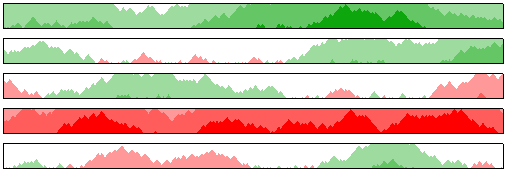
\includegraphics[width=6.5cm]{figures/horizon-new.eps}
	\caption{Five horizon graphs using green for values above the mid-line.}
	\label{fig:newHorizon}
\end{figure}

We have also proposed a different color scheme for the horizon graph, shown in Figure~\ref{fig:newHorizon}, because it can be difficult to remember the meaning of the traditional colors.  If one thinks of a temperature color scale, then red is associated with higher values and blue with lower values, which is the opposite of their intended meanings for horizon graphs.  Users already require instruction and practice to interpret the bands properly, so it would be helpful for them if the colors were less ambiguous.  Therefore, we have replaced blue with green, shown in Figure~\ref{fig:newHorizon}, so that perhaps users will be reminded of the usual financial meanings for these colors: green for above some threshold and red for below it.

The tasks from Javed et al.'s study where used in our experiment, except for the discrimination task \cite{javed2010}.  This was omitted because it seemed unrelated to how time series are read in reality.  Typically, users are concerned with how time series compare at the same point in time or across the same time range.  The discrimination task asked users to compare time series at different times, which we felt was unusual.

\subsection{Display}

All experimentation was conducted on a standard Dell desktop computer with a 20-inch monitor set to 1280 by 1024 pixels resolution.  The portion of the display where the time series were drawn occupied 500 by 515 pixels (approximately 5 by 5.25 inches).  Participants sat so their eyes were approximately 18 inches from the screen.

\subsection{Procedure}

The evaluation consisted of blocks of ten trials, one for each task with each visualization type.  This made for a total of 60 trials per participant.  A trial showed fifteen time series, from which the user selected an answer.  Each time series had a small box drawn next to it, as shown in Figure~\ref{fig:stackedGraph}, which the participant clicked to submit a response.  Response times and correctness of response were recorded.

\subsection{Tasks}

Both tasks involved selecting one time series out of set of fifteen.  The two tasks used were based on the tasks by Javed et al. \cite{javed2010}:
\begin{enumerate}
\item \textbf{Maximum:} We asked the user to identify the time series with the highest value at a given point in time that was marked on all time series.  The time was randomly chosen for each trial so it was no closer than 10\% from the beginning or end of the chart.
\item \textbf{Slope:} Two times were marked on all time series.  The user was instructed to identify the time series which increased the most from the first marked time to the second marked time.  As with the maximum task, these times were randomly chosen so that they were no closer than 10\% from the beginning or the end of the chart.  Furthermore, the distance between the two times was designed to be at least 25\% the width of the chart.
\end{enumerate}

\subsection{Conditions}

The only condition that varied in our study was the visualization type.  Our fifteen time series were represented in one of the following ways:

\begin{itemize}
\item \textbf{Small multiples:} one line chart per time series, with the area between the values and the $x$-axis filled. The same $y$-axis scale was used across all charts.  Each chart was 500 by 26 pixels.
\item \textbf{Horizon graphs:} one three-band horizon graph per time series using the red-green color scheme.  The baseline was set to the average of the global minimum and global maximum values of all time series.  The same $y$-axis scale was used across all charts.  Each chart was 500 by 26 pixels.
\item \textbf{Stacked graphs:}  one semi-transparent line chart per time series, with the area between the values and the $x$-axis filled with a texture. Each chart starts at one-fourth up the height of the previous chart. The same $y$-axis scale was used across all charts.  Each chart was 500 by 115 pixels.
\end{itemize}

\subsection{Subjects}

Four volunteers were used as subjects.  All four were graduate students in Computer Science at the University of New Hampshire.  Their vision was either 20-20 vision or corrected to 20-20 with glasses.

\section{Results}

\begin{figure}
	\begin{subfigure}[b]{0.5\textwidth}
	\footnotesize
		\begin{center}
		  \begin{tabular}{ | r | l | l | }
		    \hline
		     & \multicolumn{2}{ |c| }{Task} \\  \cline{2-3}
		     & Maximum & Slope \\ \hline
		    Small Multiples & 0.15  & 0.5 \\ \hline
		    Horizon Graphs  & 0.125 & 0.625 \\ \hline
		    Stacked Chart   & 0.65  & 0.7 \\
		    \hline
		  \end{tabular}
		\end{center}
		\caption{The percent error (out of 1.0).}
		\label{tab:resultsError}
        \end{subfigure}
	\begin{subfigure}[b]{0.5\textwidth}
	\footnotesize
		\begin{center}
		  \begin{tabular}{ | r | l | l | }
		    \hline
		     & \multicolumn{2}{ |c| }{Task} \\  \cline{2-3}
		     & Maximum & Slope \\ \hline
		    Small Multiples & 6.58  & 15.41 \\ \hline
		    Horizon Graphs  & 6.67 & 21.18 \\ \hline
		    Stacked Chart   & 19.98  & 20.57 \\
		    \hline
		  \end{tabular}
		\end{center}
		\caption{Mean response time (seconds).}
		\label{tab:resultsTime}
        \end{subfigure}
	\caption{The results of the evaluation.}
	\label{tab:results}
\end{figure}

The results of our evaluation are shown in tabular form in Figure~\ref{tab:results} and as charts in Figure~\ref{fig:results}.  We have recorded and calculated the mean response time and percent error; smaller values are desired for both.  The results show that the slope task seems to have been much more difficult than the maximum task for all three chart types since the times approximately doubled from the maximum task.  Small multiples seem to have been slightly better suited to the slope task, but the mean response times and errors were fairly similar across the different chart types.  Horizon graphs led to slightly lower errors than small multiples for the maximum task, though they were fairly equivalent and both were much better than stack graphs in terms of time and error.  For both tasks, the stacked charts proved to have high errors and high response times.

\section{Discussion}

There were only slight differences between the chart types for the slope task, but the stacked graph proved to be inefficient for the maximum task, attaining an error---0.65---over four times as a high as the other chart types.  Furthermore, response times were approximately three times higher for the stacked graph with the maximum task, meaning participants took longer to reach the wrong answer for the stacked graph.  This matches with the commentary provided by the different participants following completion of the evaluation; the stacked graphs were described as ``confusing'' and ``a mess.''

\begin{figure}
	\begin{subfigure}[b]{0.49\textwidth}
		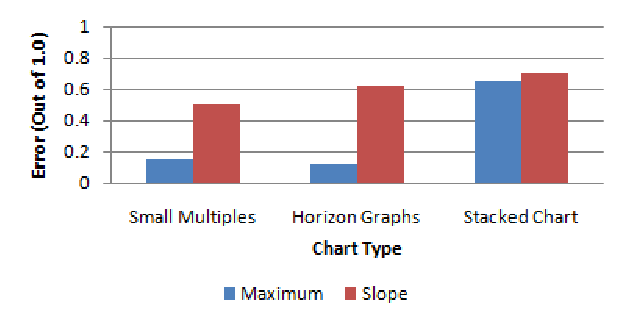
\includegraphics[width=\textwidth]{figures/results-error.eps}
		\caption{The percent error (out of 1.0).}
		\label{fig:resultsError}
        \end{subfigure}
	\begin{subfigure}[b]{0.49\textwidth}
		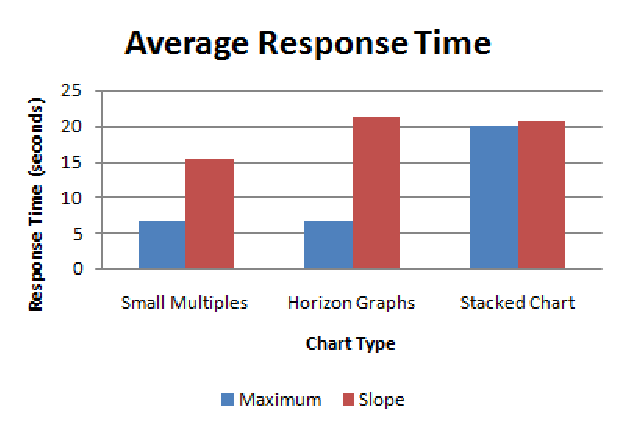
\includegraphics[width=\textwidth]{figures/results-time.eps}
		\caption{Mean response time (seconds).}
		\label{fig:resultsTime}
        \end{subfigure}
	\caption{The results of the evaluation graphed.}
	\label{fig:results}
\end{figure}

These results seem to show that the stacked graph is inferior to the horizon graph and small multiples and should, therefore, be avoided when plotting many concurrent time series.  While this may be true, it could also be possible that our implementation was suboptimal.  In the design phase, we incrementally attempted to improve the colors and textures used for the stacked graphs.  However, there may be other color and texture combinations that would lead to a better performance.  Also, it is possible that a different vertical offset could lead to better results.

There were major differences between the two tasks---maximum task and slope task---for the small multiples and horizon graphs.  Both chart types had reasonably low errors and response times for the maximum task, but much higher errors and times for the slope task.  There could be a number of possible explanations for this---e.g., none of these chart types are suited to this task, the task is too complicated with fifteen time series at once, or the task was improperly explained to participants.  More research would be required to determine the reason for the overall difficulty with the slope task.

\subsection{Conclusion}

Our study disproved our hypothesis unfortunately; for these tasks, the stacked graph seemed to be inefficient and, worse, misleading for representing many time series.  Small multiples or horizon graphs were much better for the two tasks involved and seemed to be fairly equivalent to each other.  When representing several concurrent time series, we recommend using either small multiples or horizon graphs.  To chose between the two chart types, one may follow Javed et al.'s recommendations, which found small multiples to be more robust than horizon graphs \cite{javed2010}.  Adjustments to the coloring and texturing of the stacked graph may lead to improvements, though these changes should be evaluated before being used in practice.

\subsection{Future Work}

There are many different combinations of color and texture possible for use with a stacked graph, some of which might lead to improvements.  Furthermore, additional techniques such as fading opacity could be used to enhance the stacked graph's appearance.

Our idea to use a red-green color scheme for the horizon graph leads to the question: what color scheme is best for the understandability of the horizon graph?  Previous evaluations on the horizon graph have focused on the overall size of the chart or the number of overlapping bands; perhaps it might be useful to evaluate different color schemes for the horizon graph.

\bibliographystyle{plain}

\bibliography{sources}

\end{document}
